\documentclass[tikz]{standalone}
\usepackage{pgfplots}
\pgfplotsset{compat=1.15}
\usepackage{mathrsfs}
\usetikzlibrary{arrows,calc}
\usepackage{tkz-euclide}

\pagestyle{empty}

\definecolor{AngleClr}{rgb}{0,0.39215686274509803,0}
\definecolor{ShapeClr}{rgb}{0.6,0.2,0}
\definecolor{BlueClr}{RGB}{5,81,163}

\begin{document}

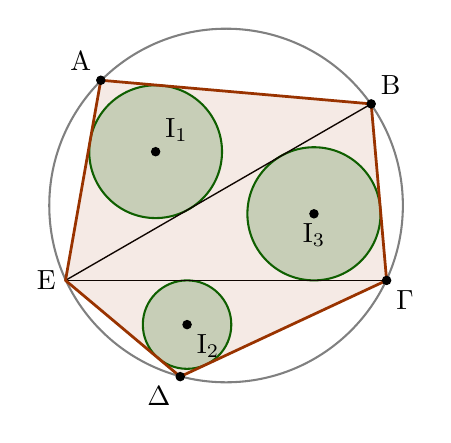
\begin{tikzpicture}[scale=.75]
\tkzSetUpLine[line width=1pt,color=black]
\tkzSetUpPoint[fill=black]

\tkzDefPoint(135:3){A}
\tkzDefPoint(35:3){B}
\tkzDefPoint(-25:3){C}
\tkzDefPoint(-105:3){D}
\tkzDefPoint(-155:3){E}


\tkzDefTriangleCenter[circum](A,B,C) \tkzGetPoint{O}

\tkzDefCircle[in](A,B,E) \tkzGetPoints{I1}{i1}
\tkzDefCircle[in](C,D,E) \tkzGetPoints{I2}{i2}
\tkzDefCircle[in](B,C,E) \tkzGetPoints{I3}{i3}
\tkzDrawCircles[color=AngleClr,fill=AngleClr,fill opacity=0.2,line width=0.75](I1,i1 I2,i2 I3,i3)


\tkzDrawCircle[line width=0.75](O,A)

\tkzDrawSegments[line width=0.5pt,color=black](B,E C,E)

\tkzFillPolygon[fill=ShapeClr,fill opacity=0.1](A,B,C,D,E)
\tkzDrawPolygon[color=ShapeClr](A,B,C,D,E)


\tkzDrawPoints[size=3](A,B,C,D,I1,I2,I3)
\tkzLabelPoint[above left](A){$\rm A$}
\tkzLabelPoint[above right](B){$\rm B$}
\tkzLabelPoint[below right](C){$\rm \Gamma$}
\tkzLabelPoint[below left](D){$\rm \Delta$}
\tkzLabelPoint[left](E){$\rm E$}

\tkzLabelPoint[above right](I1){$\rm I_1$}
\tkzLabelPoint[below right](I2){$\rm I_2$}
\tkzLabelPoint[below](I3){$\rm I_3$}


\end{tikzpicture}

\end{document}
